{The length $\ell$ of a long wall is to be approximated. The angle $\theta$, as shown in the diagram (not to scale), is measured to be $85^\circ$, and the distance $x$ is measured to be 30'. Assume that the triangle formed is a right triangle.\\

Is the measurement of the length of $\ell$ more sensitive to errors in the measurement of $x$ or in $\theta$?

\begin{minipage}{\linewidth}
\centering
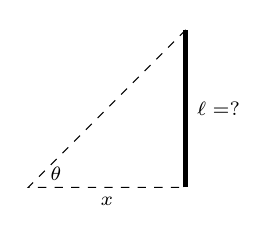
\begin{tikzpicture}
\draw [ultra thick] (1,-1) -- node [pos=.5,right] {\scriptsize $\ell=$?}(1,1);
\draw [dashed] (1,1) -- (-1,-1) node [xshift=10pt,yshift=5pt] {\scriptsize $\theta$} -- node [pos=.5,below] {\scriptsize $x$} (1,-1);
%\draw (-.5,0) -- node [pos=.5,draw=white,fill=white] {\scriptsize $50'$} (1,0);
\end{tikzpicture}
\end{minipage}
}
{Using trigonometry, $\ell = x\tan\theta$, so $d\ell = \tan\theta dx + x\sec^2\theta d\theta$. With $\theta = 85^\circ$ and $x=30$, we have $d\ell = 11.43dx+3949.38d\theta$. The measured length of the wall is much more sensitive to errors in $\theta$ than in $x$. While it can be difficult to compare sensitivities between measuring feet and measuring degrees (it is somewhat like ``comparing apples to oranges''), here the coefficients are so different that the result is clear: a small error in degree has a much greater impact than a small error in distance.
}